\documentclass{article}
\usepackage[margin=0.6in]{geometry}
\usepackage[utf8]{inputenc}
\usepackage{physics}
\usepackage{graphicx}
\usepackage{siunitx}
\usepackage{amsmath}
\usepackage{amssymb}
\usepackage[dvipsnames]{xcolor}
\usepackage[sort&compress]{natbib}
\usepackage{bm}
\usepackage{url}
\usepackage{hyperref}
\usepackage{parskip}
\usepackage{lineno}
\usepackage{float}
\usepackage{gensymb}
\usepackage{appendix}
\linenumbers

\setlength\parindent{0pt}
\renewcommand{\baselinestretch}{1.5}

\newcommand{\TODO}[1]{\todo[inline,backgroundcolor=red!25,bordercolor=red]{#1}}
\newcommand{\alan}[2][]{\todo[color=green, #1]{\textbf{Alan}: #2}}
\newcommand{\henri}[2][]{\todo[color=orange, #1]{\textbf{Henri}: #2}}
\usepackage[obeyFinal,textsize=footnotesize]{todonotes}


\usepackage{authblk}

\title{Optimal time-dependent deployments of climate controls}
\author[1,2]{Henri F. Drake\textsuperscript{*}}
\author[1]{Ron Rivest}
\author[1]{Alan Edelman}
\author[1]{John Deutch}
\affil[1]{Massachusetts Institute of Technology, Cambridge, MA, USA}
\affil[2]{Woods Hole Oceanographic Institution, Woods Hole, MA, USA}

\date{}             %% if you don't need date to appear
\setcounter{Maxaffil}{0}
\renewcommand\Affilfont{\itshape\small}

\begin{document}
\maketitle

\section{Background and motivation}

Ever since climate scientists began understanding how anthropogenic emissions of greenhouse gases and aerosols have unintentionally altered Earth's climate \citep{manabe1967thermal, schneider_carbon_1975, broecker_climatic_1975}, they have speculated about the intentional manipulation of such mechanisms for climate control \citep[][and references therein]{kellogg_climate_1974}.
% Review of climate change science and model hierarchy

% Climate controls: roles of mitigation, carbon dioxide removal, adaptation, and solar geoengineering

% , either by afforestation, soil carbon sequestration, direct air capture, bio-energy and carbon capture and sequestration, or enhanced weathering (see reviews of \citealt{minx_negative_2018, fuss_negative_2018}).

% Review of IAMs and limitations

% Role of models in climate policy

% Summary of our approach

Coming soon.

\alan[inline]{Nice to mention En-Roads, and mention that
it also seeks to raise consciousness }

\section{An Idealized Model for Optimal Climate Control}

The MARGO model consists of a physical energy balance model of Earth's climate, an idealized model of climate damages and controls:
\begin{center}
\begin{tabular}{l}
\textbf{M}itigation of greenhouse gas emissions, \\
\textbf{A}daptation to climate impacts, \\
\textbf{R}emoval of carbon dioxide, \\
\textbf{G}eoengineering by radiation management,
\end{tabular}
\end{center}
and a modular, fast, and customizable \textbf{O}ptimization model with several options of objective functions and constraints. 
\henri[inline]{Other naming options are ARMS (Adaptation Removal Mitigation Solar-geoengineering), ....}

Each of the climate controls acts, in its own distinct way, to reduce the damages caused by  changing climate but also carry their own deployment costs (including research and development costs, infrastructure costs, political costs, costs of side-effect damages, etc). The model is designed to include key features of climate physics, economics, and policy as concisely as possible and in ways qualitatively consistent with both fundamental theory and more comprehensive models. We aim to construct a model which yields fundamental insights into optimal management of climate change but is significantly more accessible, transparent, flexible, and computationally inexpensive than conventional models. The model is developed in open source using the Julia programming language \citep{bezanson_julia:_2017} at \href{github.com/hdrake/OptimizeClimate}{github.com/hdrake/OptimizeClimate} (Drake et al., 2020). The parameter values used throughout the paper are set to the defaults in Tables \ref{tab.parameters} and \ref{tab.controls}, except where explicitly stated otherwise, and are justified in Section \ref{sec.parameters}. In Appendix \ref{}, we show that by tweaking just a handful of these default parameter values, the model replicates the qualitative results from studies ranging from analytical control theory analysis \citep{soldatenko_optimal_2018} to numerical optimizations of commonly used Integrated Assessment Models such as DICE \citep{belaia_optimal_2019}.

\subsection{CO$_{2}$ concentrations: baseline emissions, emissions reductions, and negative emissions}

In the absence of climate policy, we assume CO$_{2}$ concentrations in the model start at present values of $c_{0} \equiv c(t_{0})$ in $t_{0}=2020$ CE and increase according to a baseline emissions scenario $q(t)$. The baseline concentrations are given by the accumulation of emissions in the atmosphere,
\begin{equation}
c(t) = c_{0} + \int_{t'=t_{0}}^{t} rq(t') \text{ d}t',
\end{equation}
where $r \approx 40\%$ is the fraction of emissions which remain in the atmosphere, net of uptake by the terrestrial biosphere and the ocean \citep{solomon_irreversible_2009}, and $rq(t)$ are the \textit{effective emissions} that contribute to planetary warming via the greenhouse effect. The model currently has no explicit carbon cycle but in the future will include an idealized dynamic ocean carbon cycle \citep{glotter_simple_2014}, which captures both the initial linear uptake of carbon by the ocean and non-linear feedbacks due to the ocean's limited chemical buffering capacity. While we here only explicitly model CO$_{2}$ effects, other greenhouse gases may be approximated by forcing the model with the CO$_{2}$ concentrations that result in the equivalent global-mean forcing from all greenhouse gases, referred to as carbon dioxide-equivalent concentrations CO$_{2e}$. The radiative effects of aerosols (and other minor anthropogenic effects) are similarly bundled into CO$_{2e}$ but could instead be prescribed as additional time-dependent global-mean forcing terms, with associated damages (e.g. the negative health effects of airborne particulate matter) which could in turn be reduced by abatement policies \citep{thompson_systems_2014}.

For simplicity, we calibrate our baseline effective emissions to the no-climate-policy Representative Concentration Pathway (RCP) 8.5, which results in $\SI{8.5}{W m^{-2}}$ of radiative forcing by 2100 relative to preindustrial levels, mostly due to greenhouse gas emissions from rampant fossil fuel consumption \citep{riahi_scenarios_2007}. We approximate the RCP8.5 emissions by the continuous and piecewise linear function:
\begin{equation}
    q(t) = 
    \begin{cases}
        q_{0}(1 + 2\frac{2100-t}{2100-2020}) &\mbox{if } t \le \SI{2100}{CE} \\
        3q_{0}\frac{2150-t}{2150-2100} &\mbox{if } \SI{2100}{CE} < t \le \SI{2150}{CE} \\
        0 &\mbox{if } \SI{2150}{CE} < t
    \end{cases},\label{eq.baseline_emissions}
\end{equation}
in which CO$_{2e}$ emissions increase linearly from a present-day value $q_{0} = \SI{10}{ppm\, yr^{-1}}$ ($\SI{50}{GtCO_{2e}\, yr^{-1}}$) to a maximum of $3q_{0} = \SI{30}{ppm\, yr^{-1}}$ in $\SI{2100}{CE}$ and then decrease linearly to zero by $\SI{2150}{CE}$ (Figure \ref{fig.temp_and_carbon}a). These effective emissions $rq(t)$ result in CO$_{2e}$ concentrations of about $\SI{1400}{ppm}$ and a corresponding anthropogenic radiative forcing of $\SI{8.5}{W\, m^{-2}}$ by $\SI{2150}{CE}$, relative to preindustrial levels (see below).

CO$_{2}$ emissions reductions are parameterized by the fractional \textbf{M}itigation of annual emissions $M(t) \in [0,1]$ such that the net annual emissions become $q(1-M(t))$. In acknowledgement of existing mitigation policies that make our current trajectory diverge from RCP8.5, we assume weak present day mitigation of $M(t_{0}) = \SI{5}{\%}$ \citep{hausfather_emissions_2020}.

CO$_{2}$ \textbf{R}emoval is parameterized by the fraction $R(t) \in [0,1]$ of the baseline emissions $q_{0}$ in $\SI{2020}{CE}$ that are sequestered from the atmosphere in a given year. The CO$_{2}$ concentrations in a given year are thus given by (Figure \ref{fig.temp_and_carbon}b):
\begin{equation}
    c_{M, R}(t) = c_{0} + \int_{t'=t_{0}}^{t} r(1-M(t'))q(t') - R(t')q_{0} \text{ d}t'\label{eq-CO2-conc},
\end{equation}
where $c_{0} \equiv c(t_{0}) \approx \SI{460}{ppm}$ is roughly the present CO$_{2e}$ concentration. Figures \ref{fig.temp_and_carbon}a,b show the effective CO$_{2e}$ emissions and concentrations, respectively, for both the baseline scenario and an example controlled scenario.

The anomalous heat trapped by CO$_{2}$, hereafter ``radiative forcing", is theoretically and empirically found to be a logarithmic function of CO$_{2}$ concentrations
\begin{equation}
    F(t) = a \ln(\frac{c(t)}{c_{0}}),
\end{equation}
relative to $t_{0} = \SI{2020}{CE}$ and where $a \approx \SI{4.97}{W m^{-2}}$. The controlled greenhouse forcing is similarly given by:
\begin{equation}
    F_{M, R}(t) = a \ln(\frac{c_{M, R}(t)}{c_{0}}).
\end{equation}

The controlled greenhouse radiative forcing $F_{M, R}$ is (optionally) partially offset by Solar-\textbf{G}eoengineering measures, which reduce the amount of solar energy absorbed by the surface and consequently impose a negative radiative forcing
\begin{equation}
F_{G}(t) \equiv -G(t)F(t \rightarrow \infty)
\end{equation}
determined by the fraction $G(t) \in [0,1]$ of the ultimate greenhouse forcing  $F(t \rightarrow \infty) = \SI{8.5}{W\, m^{-2}}$ that is offset by controlling solar radiation. The controlled net radiative forcing is thus given by:
\begin{equation}
    F_{M, R, G}(t) = F_{M, R}(t) + F_{G}(t).
\end{equation}

\begin{figure}[htb!]
\noindent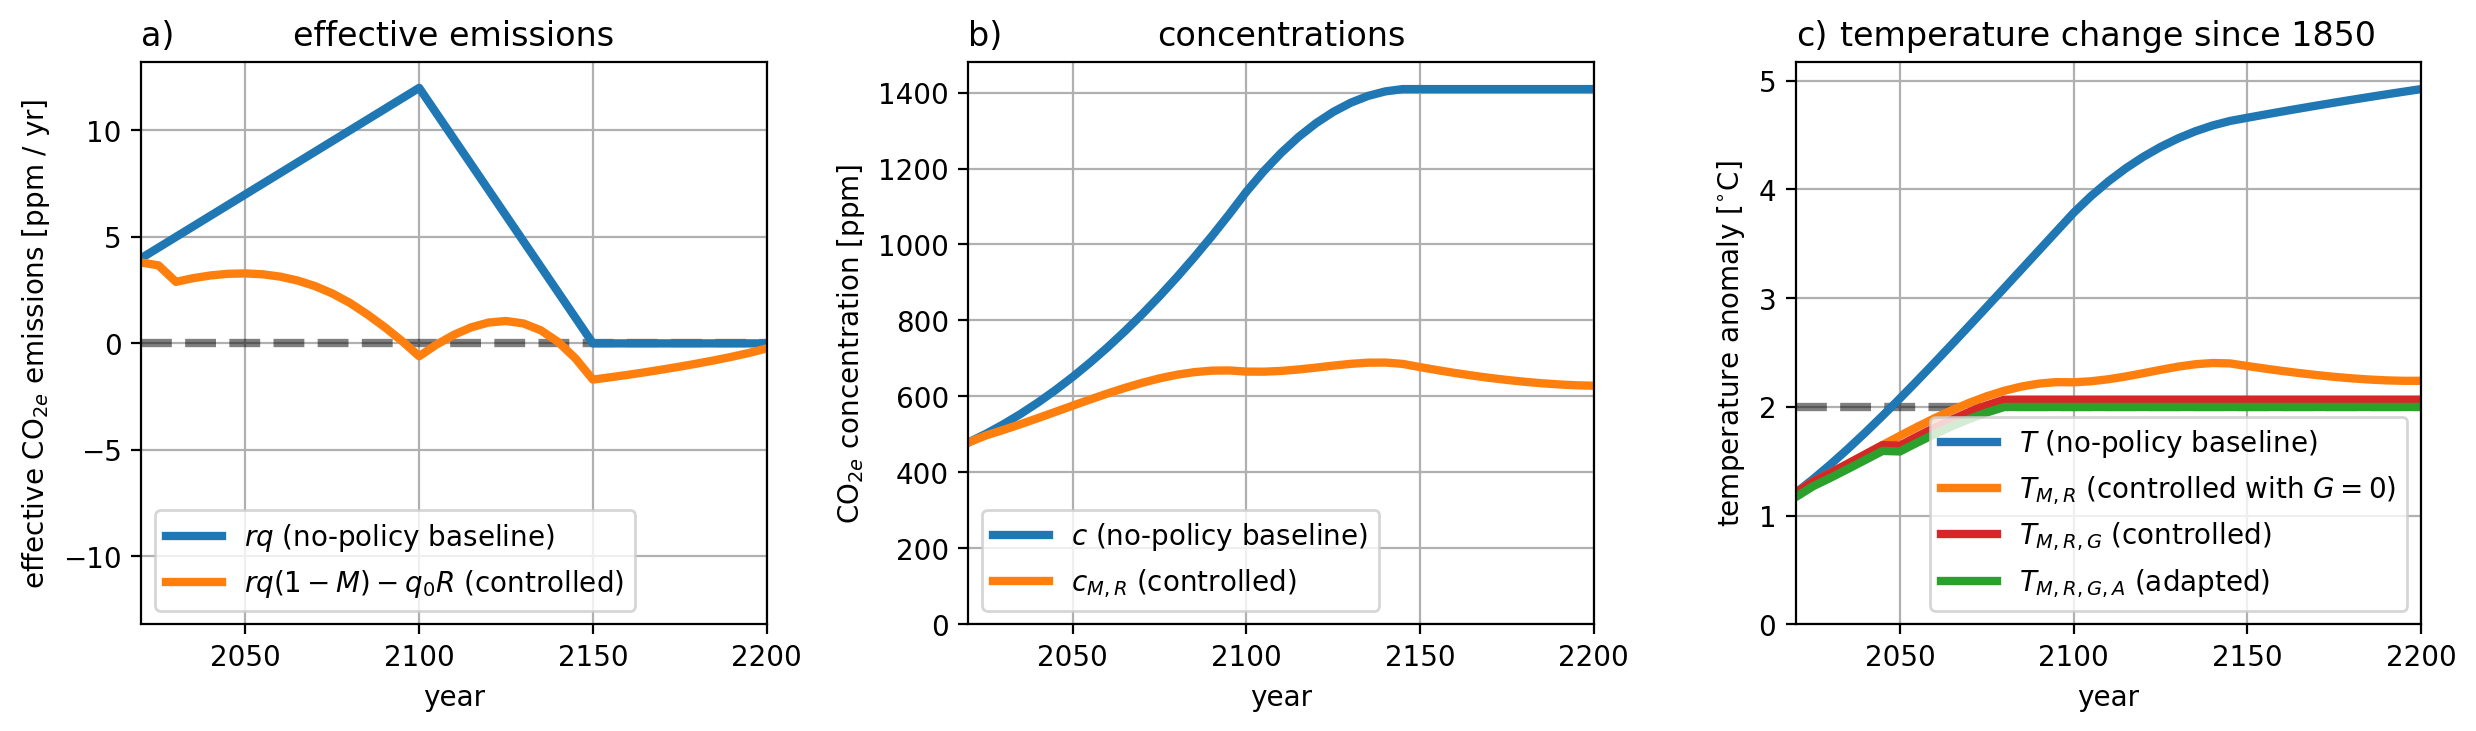
\includegraphics[width=1.0\textwidth]{figures/default-temp_carbon_and_temperatures.png}
\centering
\caption{Baseline (blue) and optimal (orange) a) effective CO$_{2}$ emissions, b) CO$_{2}$ concentrations, and c) temperature anomaly relative to preindustrial from cost-effectiveness analysis (see Section \ref{sec.cost-effectivness}). Panel c) shows the optimal temperature change that would occur: in a baseline scenario (blue); with just emissions \textbf{M}itigation and carbon dioxide \textbf{R}emoval (orange); with \textbf{M}itigation, \textbf{R}emoval, and solar-\textbf{G}eoengineering (red); and as an ``adapted temperature" (eq. \ref{eq.adapted_temperature}) with \textbf{A}daptation measures also taken into account. The dashed grey line marks the threshold temperature of $\SI{2}{\celsius}$ to be avoided.}
\label{fig.temp_and_carbon}
\end{figure}

\subsection{Temperature response to CO$_{2}$ forcing}
The evolution of the global-mean near-surface temperature anomaly (relative to the initial time $t_{0} = \SI{2020}{CE}$) is determined by the two-box linear energy balance model \citep[e.g][]{gregory_vertical_2000, held_probing_2010}:
\begin{gather}
    C_{U} \dv{T}{t} = -B T - \kappa( T - T_{D}) + F(t), \label{eq.upper_ocean}
    \\
    C_{D} \dv{T_{D}}{t} = \kappa (T - T_{D}),\label{eq.deep_ocean}
\end{gather}
where (\ref{eq.upper_ocean}) represents the upper ocean with average temperature anomaly $T$, and (\ref{eq.deep_ocean}) represents the deep ocean with an average temperature $T_{D}$. The near-surface atmosphere exchanges heat rapidly with the upper ocean and thus the global-mean near-surface air temperature is also given by $T$. The model parameters are: the upper ocean heat capacity $C_{U}$ (including a negligible contribution $C_{A} \ll C_{U}$ from the atmosphere); the deep ocean heat capacity $C_{D}$; the climate feedback parameter $B$; the ocean mixing rate $\kappa$; and $F(t)$ the anomalous anthropogenic radiative forcing. The radiative forcing and temperature anomalies at $t_{0} = \SI{2020}{CE}$ relative to preindustrial are $F(t_{0}) - F(t_{\text{pre}}) = \SI{2.5}{W\, m^{-2}}$ and $T_{0} \equiv T(t_{0}) - T(t_{\text{pre}}) = \SI{1.1}{K}$, where we set $F_{0} \equiv F(t_{0}) = \SI{0}{W\, m^{-2}}$ and $T(t_{\text{pre}}) = \SI{0}{K}$ for convenience.

Since, by construction, the anthropogenic forcing $F(t)$ varies on timescales longer than the fast relaxation timescale $\tau_{U} = C_{U}/(B + \kappa)$, we can ignore the time-dependence in the upper ocean and approximate
\begin{equation}
    T \approx \frac{F+\kappa T_{D}}{B + \kappa},
    \label{eq.shallow_approx}
\end{equation}
where the evolution of the deep ocean
\begin{equation}
    C_{D} \dv{T_{D}}{t} \approx - \frac{B \kappa}{B + \kappa} T_{D} + \frac{\kappa}{B + \kappa} F
    \label{eq.deep_ode}
\end{equation}
occurs on a slower timescale $\tau_{D} \equiv \dfrac{C_{D}}{B} \dfrac{B + \kappa}{\kappa}$ \citep{held_probing_2010}. Plugging the exact solution to (\ref{eq.deep_ode}) into (\ref{eq.shallow_approx}) gives the integral solution
\begin{equation}
    T(t) - T_{0} = \frac{F(t)}{B + \kappa} + \frac{\kappa}{B} \frac{1}{(B+\kappa)} \int_{t_{0}}^{t} \frac{ e^{-(t-t')/\tau_{D}}}{\tau_{D}} F(t') \, \text{d}t'.\label{eq.baseline_temperature}
\end{equation}
The evolution of the controlled temperature anomaly (Figure \ref{fig.temp_and_carbon}c)
\begin{equation}
    T_{M,R,G}(t) - T_{0} =  \frac{F_{M,R,G}(t)}{B + \kappa} + \frac{\kappa}{B} \frac{1}{(B+\kappa)} \int_{t_{0}}^{t} \frac{ e^{-(t-t')/\tau_{D}}}{\tau_{D}} F_{M,R,G}(t') \, \text{d}t'\label{eq.temperature}
\end{equation}
is thus driven by the controlled net radiative forcing $F_{M,R,G}$.

We identify the first term on the right hand side of (\ref{eq.baseline_temperature}) and (\ref{eq.temperature}) as the transient climate response \citep{gregory_transient_2008}, which dominates for $t-t_{0} \ll \tau_{D}$, while the second term is a slower ``recalcitrant" response due to a weakening of ocean heat uptake as the deep ocean comes to equilibrium with the transiently warmer upper ocean \citep{held_probing_2010}. While the contribution of the recalcitrant component to historical warming is thought to be small, it contributes significantly to 21st century and future warming \citep{gregory_transient_2008,held_probing_2010}. If the instantaneous radiative forcing vanishes, as in the case of either complete decarbonization or strong solar geoengineering, the recalcitrant component is the only remaining cause of temperature change (Figure \ref{fig.temp_and_carbon}c, see also \citealt{gregory_transient_2008, held_probing_2010}).

The behavior of the model on short and long timescales is illustrated by applying it to the canonical climate change experiment in which CO$_{2}$ concentrations increase at 1\% per year until doubling. The temperature anomaly first rapidly increases until it reaches the Transient Climate Sensitivity $TCS = \dfrac{F_{2\times}}{B + \kappa}$ around the time of doubling $t=t_{2\times}$, with $t_{2\times} - t_{0} \ll \tau_{D}$ and $F_{2\times} = \alpha \ln(2)$, and then gradually asymptotes to the Equilibrium Climate Sensitivity $ECS = \dfrac{F_{2\times}}{B} > TCS$ on a much longer timescale $t-t_{0} \gg \tau_{D}$.

\subsection{Climate damages}

Annual climate damages are assumed to be of the quadratic form $D(t) = \beta T(t)^{2}$, such that successive temperature increases are increasingly damaging, based on empirical estimates of damages which range from linear to cubic functions of global-mean temperature change relative to preindustrial \citep{stern_economics_2007}. The default value of the damage parameter $\beta$ is chosen to be roughly similar to the DICE model for low levels of warming \citep{nordhaus2013dice}, resulting in damages of 2\% of global world product at \SI{2}{\celsius}.

\textbf{A}daptation to climate change impacts (e.g. building sea walls, installing air conditioning units, planting climate-resilient crops) is parameterized by reducing annual damages by a fraction $A(t) \in [0,1]$, such that the total controlled damages are:
\begin{equation}
    D_{M, R, G, A} = \beta \; (T_{M, R, G}(t))^{2} \; (1-A(t)).
\end{equation}
Although adaptation does not affect the planetary temperature directly, it is useful to consider an ``adapted temperature" $T_{M,R,G,A}$ which yields damages equivalent to the fully-controlled damages $\beta (T_{M,R,G,A})^{2} = \beta (T_{M,R,G})^{2} (1-A)$, given by
\begin{equation}
    T_{M,R,G,A} \equiv T_{M,R,G} \sqrt{(1-A)}.\label{eq.adapted_temperature}
\end{equation}
In Figure \ref{fig.temp_and_carbon}, for example, while the controlled temperature $T_{M,R,G}$ overshoots the $\SI{2}{\celsius}$ warming threshold, the ``adapted temperature" $T_{M,R,G,A}$ remains below the threshold.

\subsection{Control costs}

The annual costs of deploying climate controls is given by
\begin{equation}
    \mathcal{C}_{M, R, G, A}(t) = \sum_{\alpha \in \mathcal{A}} \mathcal{C}_{\alpha} f^{(\alpha)}(\alpha(t)),
\end{equation}
where $\mathcal{A} = \{M, R, G, A \}$ is the set of climate controls, $\mathcal{C}_{\alpha}$ is the reference cost of each climate control, and $f^{(\alpha)}(\alpha)$ is a function that determines how the deployment cost increases as a function of fractional deployment. The reference cost $\mathcal{C}_{\alpha}$ corresponds to the hypothetical cost of full deployment of that control (e.g. $\mathcal{C}_{M}$ is the cost of fully decarbonizing society). However, the reference costs may be more usefully tuned based on a smaller deployment threshold, for which costs estimates are likely to be more accurate and reflective of plausible near-future deployment fractions.

We will here assume the reference costs of mitigation $\mathcal{C}_{M}$, removal $\mathcal{C}_{R}$, and adaptation $\mathcal{C}_{A}$ are fixed in time and reflect the required investments in abatement measures. In contrast, the reference cost of geoengineering $\mathcal{C}_{G}$ is thought to be dominated by the damages due to unintended side effects rather than the direct investment in deployment and thus scales with the time-dependent global economy: $\mathcal{C}_{G}(t) = \tilde{\mathcal{C}}_{G} E(t)$, where $E(t) = E_{0}(1 + \gamma)^{(t-t_{0})}$ is the Gross World Product (GWP), determined by a fixed exogenous economic growth rate $\gamma$; and  $\tilde{\mathcal{C}}_{G}$ is the damage due to deploying $F(t \rightarrow \infty) = \SI{8.5}{W m^{-2}}$ worth of solar radiation management, as a fraction of the GWP.

We do not include learning effects beyond their possible influence in setting the shape of the deployment cost functions $f^{(\alpha)}(\alpha) = \alpha^{p_{\alpha}}$, but they could be included explicitly in the future. Here, we will focus on the medium deployment cost scenario $f(\alpha) = \alpha^{2}$ ($p_{\alpha} = 2$ for all $\alpha \in \mathcal{A}$), which has the following interpretable properties: 
\begin{itemize}
    \item $\left. \dv{f}{\alpha}\right|_{\alpha=0} = 0$ (initial marginal deployment is effectively free)
    \item $f(1) = 1$ (full deployment costs $\mathcal{C}_{\alpha}$), and
    \item $\dv[2]{f}{\alpha} > 0$ (convex, such that deployment gets progressively more and more expensive).
\end{itemize}

\subsection{Optimization Methods}

We use the Interior Point Optimizer (\href{https://github.com/coin-or/Ipopt}{https://github.com/coin-or/Ipopt}), an open source software package for large-scale nonlinear optimization, to minimize the various objective functions subject to assumed policy constraints, as described in Section \ref{sec.policy_frameworks}. In practice, the control variables $\alpha \in \mathcal{A} = \{ M, R, G, A\}$ are discretized into $N = (t_{f} - t_{0}) / \Delta t$ timesteps (default $\Delta t = \SI{5}{years}$) resulting in an $4N$-dimensional optimization problem. In the default (deterministic and convex) configuration, the model takes only $\mathcal{O}(\SI{10}{ms})$ to solve after just-in-time compiling and effectively provides user feedback in real time, making it amenable to our forthcoming interactive web application (e.g. following the lead of the impactful \href{https://en-roads.climateinteractive.org/scenario.html?v=2.7.11}{En-ROADS} model, \citealt{siegel2018roads}).

\section{Climate change policy frameworks}\label{sec.policy_frameworks}

In contrast to conventional Integrated Assessment Models, which follow classic economic theories of optimal economic growth and solve for the maximal welfare based on the discounted utility of consumption, we here treat economic growth as exogenous (ignoring economy-policy-climate feedbacks) and simply aim to minimize the costs– and maximize the benefits– of deploying climate change controls, subject to constraints from policy goals.

In Section \ref{sec.cost_benefit}, we describe a cost-benefit analysis approach which finds the trajectories of control deployments that optimize trade-offs between the costs of deploying climate controls and the benefit of avoiding climate damages due to these controls. The cost-benefit approach depends strongly on the magnitude of the poorly-constrained damage function $D(T)$, which is thought to be under-estimated by conventional bottom-up approaches \citep{ackerman_limitations_2009}. Thus, in Section \ref{sec.cost-effectivness} we also explore an alternative scenario in which we instead impose an upper bound on permissible climate damages, or temperatures (as in the 2015 United Nations Paris Agreement on Climate Change), and find the lowest cost climate control trajectories which still satisfy this constraint.

\paragraph{Policy and technology readiness constraints.} For each control $\alpha \in \mathcal{A} = \{ M, R, G, A\}$, we assert a maximum deployment rate
\begin{equation}
    \abs{\dv{\alpha}{t}} \le \dot{\alpha},
\end{equation}
to forbid implausibly aggressive deployment scenarios, and an initial or readiness condition
\begin{equation}
    \alpha(t < t_{\alpha}) = \alpha_{0},
\end{equation} where typically $\alpha_{0} = 0$ and $t_{\alpha} \ge t_{0}$ is the earliest time at which the control is ``ready" to be deployed. In particular, in the default configuration we set $t_{R} = 2030$ CE and $t_{G} = 2050$ CE because these socio-technological systems do not yet exist at a climatically-significant scale \citep{minx_negative_2018, flegal_solar_2019}. Additionally, we interpret adaptation deployment costs as buying insurance against future damages at a fixed annual rate $\mathcal{C}_{A} f^{(A)}(A)$, with $\dot{A} = 0$, which can be increased or decreased upon re-evaluation at a later date (see Section \ref{sec.reactive}).

\paragraph{Discount rates.} A common economic assumption is that society discounts future costs and benefits relative to the present by a multiplicative discount factor $(1 + \rho)^{-(t-t_{0})}$, determined by the utility discount rate $\rho$ \citep[e.g. see reviews in][]{broome_discounting_1994, stern_economics_2007}. Ethical justifications for applying a non-zero discount rate to the multi-generational timescales of climate change are unconvincing and controversial even among economists \citep{ramsey_mathematical_1928, solow_economics_1974, stern_economics_2007}. Here we choose a discount rate of $\rho = 1\%$, on the low end of values used in literature, in the spirit of inter-generational equity\footnote{Following \cite{stern_economics_2007}'s discussion of the discount rate $\rho = \eta \frac{\dot{c}}{c} + \delta$, we argue against the use of a \textit{social discount rate} on ethical terms \citep{ramsey_mathematical_1928, solow_economics_1974}, setting $\eta \frac{\dot{c}}{c}=0$, and argue that the \textit{pure time discount rate}, the time decay rate of the probability that society exists, is small $\delta \approx 0$, such that $\rho \approx 0$. We note that while a discount rate of zero introduces a sensitivity to the length of the time period considered, the conventional use of discount rates results in an even more absurd assertion that future generations are worthless.}. 
%In Section \ref{sec.discount_rates}, we consider the sensitivity of our results to the choice of the discount rate $\rho$ and focus on the ratio $\rho / \gamma$ between the discount rate and the economic growth rate.

\subsection{Approach 1: Cost-benefit analysis}\label{sec.cost_benefit}

Here, we interpret the cost $\mathcal{C}$ of climate change as the cost of deploying climate controls to reduce climate damages while the benefits $\mathcal{B}$ are the avoided climate damages. A straight-forward solution of the cost-benefit problem is thus to minimize the difference between the time-integrated (potentially discounted) costs and benefits:
\begin{gather}
    \min \left\{ \int_{t_{0}}^{t_{f}} 
    \left(\mathcal{C}_{M, R, G, A} - \mathcal{B}_{M, R, G, A}\right) (1 + \rho)^{-(t-t_{0})} \, \text{d}t \right\}.
\end{gather}
The results of optimizing for net benefits are shown in Figure \ref{fig.approach1}. Early and aggressive emissions mitigation– and to a lesser extent carbon dioxide removal (Fig \ref{fig.approach1}a)– carry net costs of up to 750 billion USD/year relative to the baseline but deliver an order of magnitude more in benefits from 2070 to 2200 (Fig \ref{fig.approach1}b).

\begin{figure}[htb!]
\noindent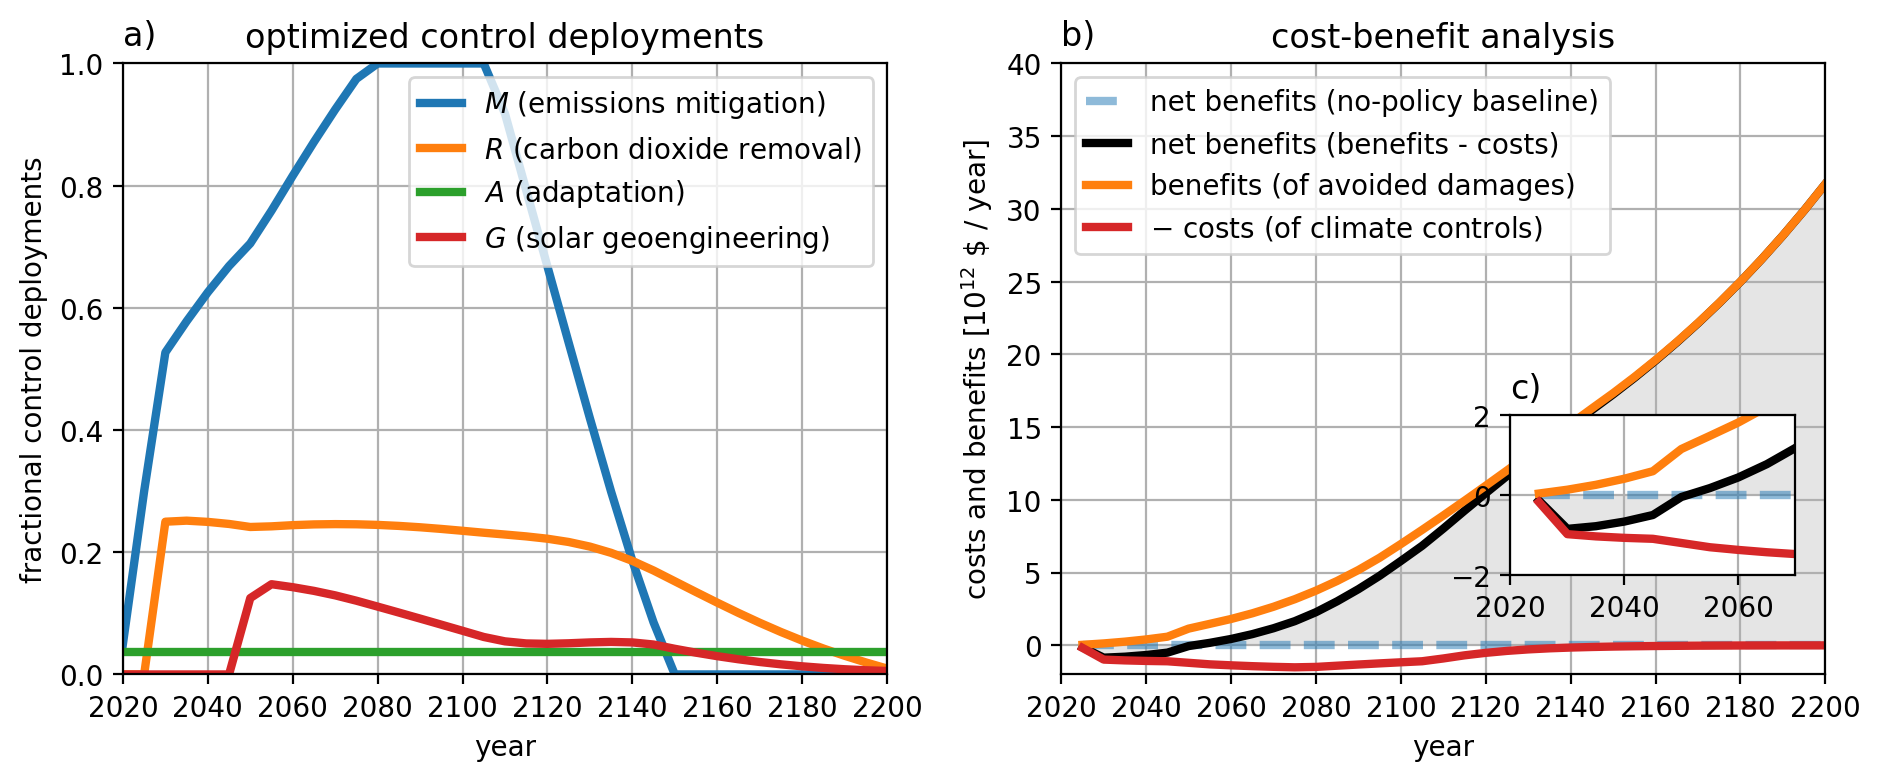
\includegraphics[width=1.0\textwidth]{figures/default-benefits_controls_and_benefits.png}
\centering
\caption{a) Optimal control deployments in a net benefit-maximizing framework and b) corresponding costs and benefits relative to a no-climate-policy baseline scenario. The total positive area shaded in grey in b) is the maximal time-integrated net benefits produced by the model.}
\label{fig.approach1}
\end{figure}

\subsection{Approach 2: Cost-effectivness of avoiding damage or temperature thresholds}\label{sec.cost-effectivness}

Coming soon (see Figure \ref{fig.approach2}).


\begin{figure}[htb!]
\noindent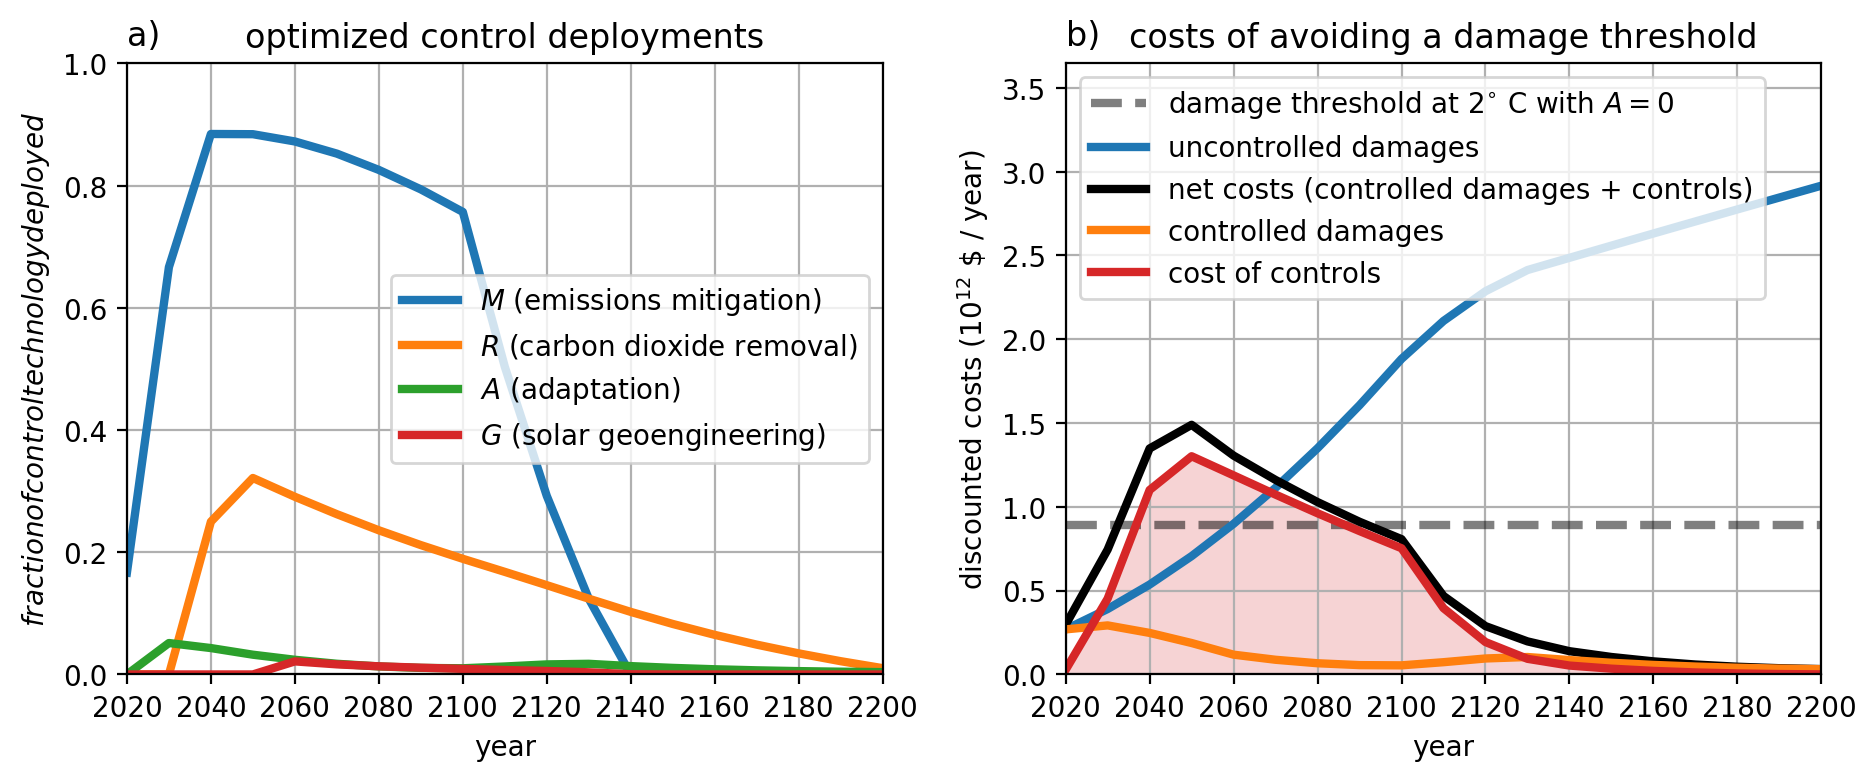
\includegraphics[width=1.0\textwidth]{figures/default-temp_controls_and_damages.png}
\centering
\caption{a) Optimal control deployments in a net cost-effectiveness framework and b) corresponding costs and damages. The total positive area shaded in red in b) is the minimal time-integrated controls costs produced by the model.}
\label{fig.approach2}
\end{figure}

\section{Designing reactive climate policy for an uncertain future}\label{sec.reactive}

Coming soon.

\begin{figure}[htb!]
\noindent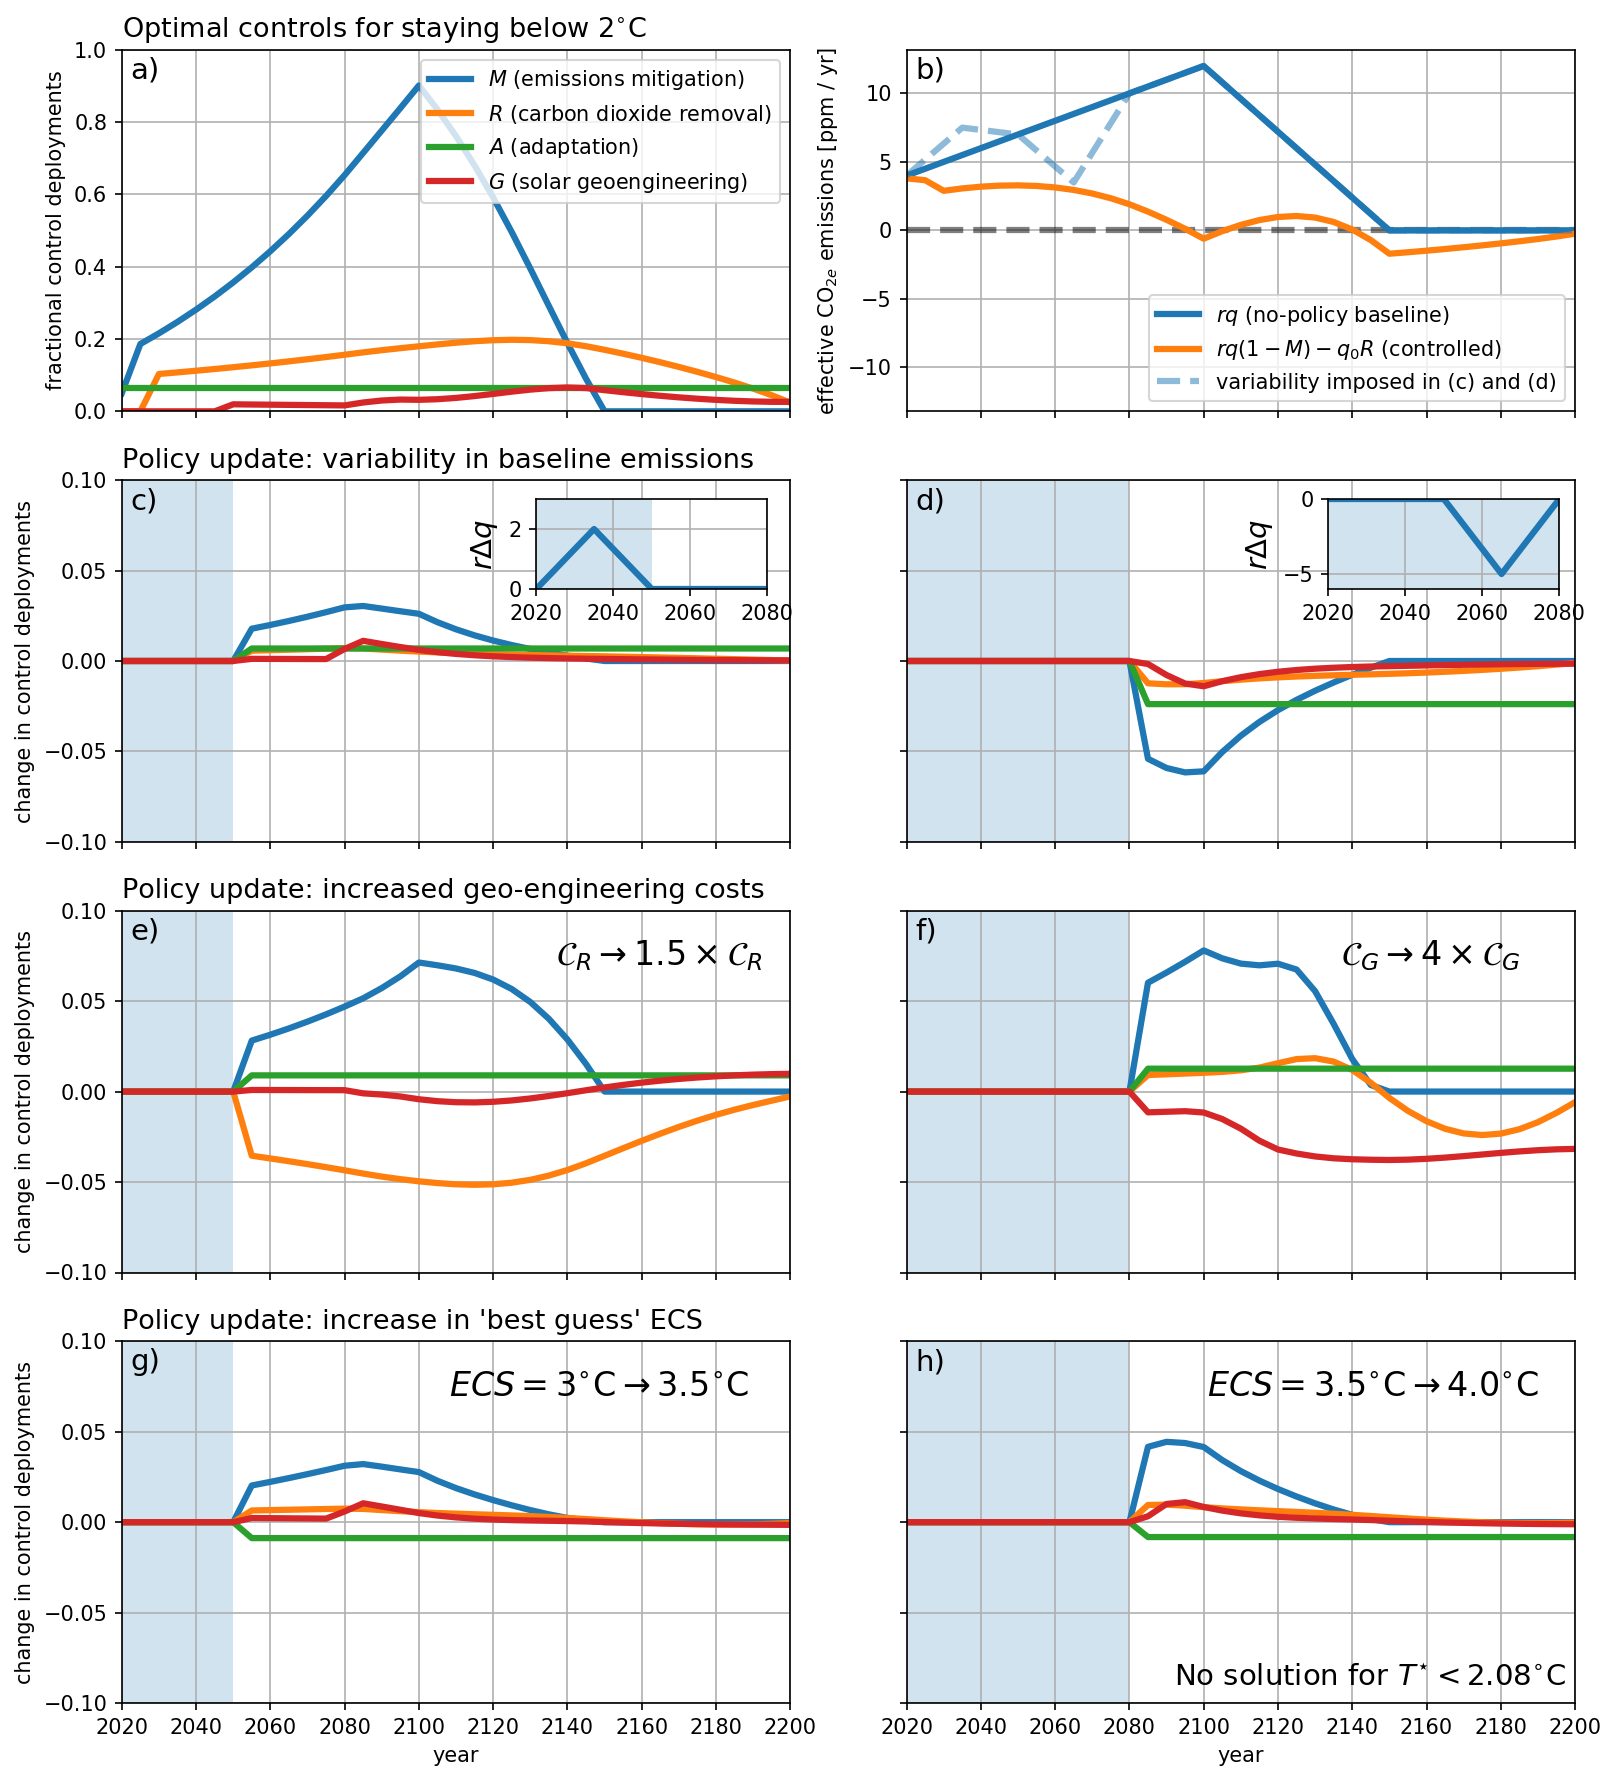
\includegraphics[width=1.0\textwidth]{figures/policy_updates.png}
\centering
\caption{}
\label{fig.policy_updates}
\end{figure}

\section{Qualitative model results}

\subsection{Extreme sensitivity to value-dependent discount rates}

\subsection{Multiple climate controls are better than one}

%\subsection{Uncertainty in climate damages strengthens the case for early action}

\section{Discussion}

Coming soon.


\appendix
\appendixpage
\addappheadtotoc

%\section{Comprehensive formulation of optimization problems}

\section{Justification and interpretation of free parameter values}\label{sec.parameters}

\subsection{Physical climate parameters}
The temperature anomaly in $t_{0}=2020$ relative to pre-industrial is roughly $T_{0} = \SI{1.1}{\celsius}$, as estimated from a global network of in-situ thermometers \citep{lenssen_improvements_2019, nasagisstemp}.

Present day CO$_{2e}(t_{0})$

The free parameters in the two-box energy balance model are set by the multi-model mean values diagnosed from the CMIP5 ensemble of general circulation climate models by \cite{Geoffr} (Tables 3 and 4). They are: the deep ocean heat capacity $C_{D} (\equiv C_{0}$), the heat exchange coefficient $\kappa (\equiv \gamma)$, and the feedback parameter $B (\equiv \lambda)$. These values are more easily interpreted with the following diagnostic variables: the Transient Climate Sensivity $TCS = \Delta F_{2\times}/(B + \kappa)$, the warming that arises shortly after a doubling of CO$_{2}$ concentrations; the Equilibrium Climate Sensitivity $ECS = \Delta F_{2\times}/B$, the equilibrium temperature anomaly due to a doubling of CO$_{2}$ concentrations, and the ocean heat uptake timescale $\tau_{D}$ which controls the asymptotic approach to the equilibrium temperature.

\subsection{Economic model parameters}

We base our reference cost for adaptation  $\mathcal{C}_{A}$ on \cite{agr2018}, which estimates annual adaptation costs of $\SI{0.5e12}{\$\, yr^{-1}}$ by 2050. They state this is likely an underestimate due to the omission of certain sectors and so set our reference cost to twice their estimate. In the face of habitability limits \citep[e.g.][]{sherwood_adaptability_2010} and exorbitant adaptation costs at high levels of warming, some unknown fraction of climate damages cannot be avoided by adaptation \citep{chambwera2014economics}; here, we impose this constraint by setting $0 \le A \le 1/3$.

\subsection{Policy action parameters}
\begin{table}[t]
\begin{center}
 \begin{tabular}{|| c || c ||}
 \hline
 Parameter & Default Configuration \\ [0.5ex] 
 \hline\hline
 $t_{0}$ & 2020 CE \\
 \hline
 $t_{f}$ & 2200 CE \\
 \hline
 $\Delta t$ & \SI{5}{yr} \\
 \hline
 $c_{0}$ & \SI{460}{ppm} \\ 
 \hline
 a & \SI{4.97}{W m^{-2}}\\
 \hline
 $q(t)$ & See eq. (\ref{eq.baseline_emissions}) \\
 \hline
 $r$ & $40\%$ \\
 \hline
 $T_{0}$ & \SI{1.1}{K} \\
 \hline
 $B$ & \SI{1.13}{W\, m^{-2}\, K^{-1}} \\
 \hline
 $\kappa$ & \SI{0.72}{W\, m^{-2}\, K^{-1}} \\
 \hline
 $C_{D}$ & \SI{106}{W\, yr\, m^{-2}\, K^{-1}} \\
 \hline
 $\beta$ & \SI{0.22e12}{\$\, yr^{-1}\, K^{-2}} \\
 \hline
 $\rho$ & $0\%$ \\
 \hline
 $E_{0}$ & \SI{100e12}{\$\, yr^{-1}}\\
 \hline
 $\gamma$ & $2\%$ \\
 \hline\hline
 \end{tabular}
\end{center}
\caption{}
\label{tab.parameters}
\end{table}

% Control parameter table
\begin{table}[t]
\begin{center}
 \begin{tabular}{|| c || c ||}
 \hline
 Parameter & Default Configuration \\ [0.5ex] 
 \hline\hline
 $M$ & $0 \le M \le 1$ \\
 \hline
 $A$ & $0 \le A \le 1/3$ \\
 \hline
 $R$ & $0 \le R \le 1$ \\
 \hline
 $G$ & $0 \le G \le 1$ \\
 \hline
 $\dot{M}$ & \SI{1/20}{yr^{-1}} \\
 \hline 
 $\dot{A}$ & \SI{0}{yr^{-1}} \\
 \hline 
 $\dot{R}$ & \SI{1/20}{yr^{-1}} \\
 \hline 
 $\dot{G}$ & \SI{1/20}{yr^{-1}} \\
 \hline 
 $t_{M}$ & $2020$ CE \\
 \hline
 $t_{A}$ & $2020$ CE \\
 \hline
 $t_{R}$ & $2030$ CE \\
 \hline
 $t_{G}$ & $2050$ CE \\
 \hline
 $M_{0}$ & $1/6$ \\
 \hline
 $A_{0}$ & $0$ \\
 \hline
 $R_{0}$ & $0$ \\
 \hline
 $G_{0}$ & $0$ \\
 \hline
 \hline
 \hline
 $\mathcal{C}_{M}$ & \SI{2e12}{\$\, yr^{-1}} \\
 \hline
 $\mathcal{C}_{A}$ & \SI{1e12}{\$\, yr^{-1}} \\
 \hline
 $\mathcal{C}_{R}$ & \SI{8.3e12}{\$\, yr^{-1}} \\
 \hline
 $\tilde{\mathcal{C}}_{G}$ & \SI{4.6}{\percent} \\ 
 \hline
 $p_{M}$ & $2$ \\
 \hline
 $p_{A}$ & $2$ \\
 \hline
 $p_{G}$ & $2$ \\
 \hline\hline
\end{tabular}
\end{center}
\caption{Values of parameters governing control variable constraints (above separation) and deployment costs (below separation).}
\label{tab.controls}
\end{table}

\bibliographystyle{apalike}
%\bibliographystyle{unsrtnat}
\bibliography{references.bib, refs_by_hand.bib}

\end{document}